
\documentclass[letterpaper,hide notes,xcolor={table,svgnames},pdftex,10pt]{beamer}
\def\showexamples{t}

\usecolortheme{crane}
\setbeamertemplate{navigation symbols}{}

\usetheme{MyPittsburgh}
\usepackage{hyperref}
\usepackage{graphicx,xspace}
\usepackage[normalem]{ulem}
\usepackage{multicol}
\usepackage{amsmath,amssymb,amsthm,graphicx,xspace}
\newcommand\SF[1]{$\bigstar$\footnote{SF: #1}}

\usepackage[sfdefault,lf]{carlito}
\usepackage[T1]{fontenc}
\usepackage[scaled]{beramono}
\usepackage{tikzpagenodes}
\newcommand{\Rplus}{\protect\hspace{-.1em}\protect\raisebox{.35ex}{\small{\small\textbf{+}}}}
\newcommand{\Cpp}{\mbox{C\Rplus\Rplus}\xspace}

\newcounter{tmpnumSlide}
\newcounter{tmpnumNote}

\newcommand\mnote[1]{%
	\addtocounter{tmpnumSlide}{1}
	\ifdefined\showcues {~\tiny\fbox{\arabic{tmpnumSlide}}}\fi
	\note{\setlength{\parskip}{1ex}\addtocounter{tmpnumNote}{1}\textbf{\Large \arabic{tmpnumNote}:} {#1\par}}}

\newcommand\mmnote[1]{\note{\setlength{\parskip}{1ex}#1\par}}


\newcommand\mquestion[2]{{~\color{red}\fbox{?}}\note{\setlength{\parskip}{1ex}\par{\Large \textbf{?}} #1} \note{\setlength{\parskip}{1ex}\par{\Large \textbf{A}} #2\par}\ifdefined \presentationonly \pause \fi}

\newcommand\blackboard[1]{%
	\ifdefined   \showblackboard
		{#1}
	\else {\begin{center} \fbox{\colorbox{blue!30}{%
						\begin{minipage}{.95\linewidth}%
							\hspace{\stretch{1}} Some space intentionally left blank; done at the blackboard.%
						\end{minipage}}}\end{center}}%
	\fi%
}

\usepackage{listings}
\lstset{%
	keywordstyle=\bfseries,
	aboveskip=15pt,
	belowskip=15pt,
	captionpos=b,
	identifierstyle=\ttfamily,
	frame=lines,
	numbers=left, basicstyle=\scriptsize, numberstyle=\tiny, stepnumber=0, numbersep=2pt}

\usepackage{siunitx}
\newcommand\sius[1]{\num[group-separator = {,}]{#1}\si{\micro\second}}
\newcommand\sims[1]{\num[group-separator = {,}]{#1}\si{\milli\second}}
\newcommand\sins[1]{\num[group-separator = {,}]{#1}\si{\nano\second}}
\sisetup{group-separator = {,}, group-digits = true}

%% -------------------- tikz --------------------
\usepackage{tikz}
\usetikzlibrary{positioning}
\usetikzlibrary{arrows,backgrounds,automata,decorations.shapes,decorations.pathmorphing,decorations.markings,decorations.text}

\tikzstyle{place}=[circle,draw=blue!50,fill=blue!20,thick, inner sep=0pt,minimum size=6mm]
\tikzstyle{transition}=[rectangle,draw=black!50,fill=black!20,thick, inner sep=0pt,minimum size=4mm]

\tikzstyle{block}=[rectangle,draw=black, thick, inner sep=5pt]
\tikzstyle{bullet}=[circle,draw=black, fill=black, thin, inner sep=2pt]

\tikzstyle{pre}=[<-,shorten <=1pt,>=stealth',semithick]
\tikzstyle{post}=[->,shorten >=1pt,>=stealth',semithick]
\tikzstyle{bi}=[<->,shorten >=1pt,shorten <=1pt, >=stealth',semithick]

\tikzstyle{mut}=[-,>=stealth',semithick]

\tikzstyle{treereset}=[dashed,->, shorten >=1pt,>=stealth',thin]

\usepackage{ifmtarg}
\usepackage{xifthen}
\makeatletter
% new counter to now which frame it is within the sequence
\newcounter{multiframecounter}
% initialize buffer for previously used frame title
\gdef\lastframetitle{\textit{undefined}}
% new environment for a multi-frame
\newenvironment{multiframe}[1][]{%
	\ifthenelse{\isempty{#1}}{%
		% if no frame title was set via optional parameter,
		% only increase sequence counter by 1
		\addtocounter{multiframecounter}{1}%
	}{%
		% new frame title has been provided, thus
		% reset sequence counter to 1 and buffer frame title for later use
		\setcounter{multiframecounter}{1}%
		\gdef\lastframetitle{#1}%
	}%
	% start conventional frame environment and
	% automatically set frame title followed by sequence counter
	\begin{frame}%
		\frametitle{\lastframetitle~{\normalfont(\arabic{multiframecounter})}}%
		}{%
	\end{frame}%
}
\makeatother

\makeatletter
\newdimen\tu@tmpa%
\newdimen\ydiffl%
\newdimen\xdiffl%
\newcommand\ydiff[2]{%
	\coordinate (tmpnamea) at (#1);%
	\coordinate (tmpnameb) at (#2);%
	\pgfextracty{\tu@tmpa}{\pgfpointanchor{tmpnamea}{center}}%
	\pgfextracty{\ydiffl}{\pgfpointanchor{tmpnameb}{center}}%
	\advance\ydiffl by -\tu@tmpa%
}
\newcommand\xdiff[2]{%
	\coordinate (tmpnamea) at (#1);%
	\coordinate (tmpnameb) at (#2);%
	\pgfextractx{\tu@tmpa}{\pgfpointanchor{tmpnamea}{center}}%
	\pgfextractx{\xdiffl}{\pgfpointanchor{tmpnameb}{center}}%
	\advance\xdiffl by -\tu@tmpa%
}
\makeatother
\newcommand{\copyrightbox}[3][r]{%
	\begin{tikzpicture}%
		\node[inner sep=0pt,minimum size=2em](ciimage){#2};
		\usefont{OT1}{phv}{n}{n}\fontsize{4}{4}\selectfont
		\ydiff{ciimage.south}{ciimage.north}
		\xdiff{ciimage.west}{ciimage.east}
		\ifthenelse{\equal{#1}{r}}{%
			\node[inner sep=0pt,right=1ex of ciimage.south east,anchor=north west,rotate=90]%
			{\raggedleft\color{black!50}\parbox{\the\ydiffl}{\raggedright{}#3}};%
		}{%
			\ifthenelse{\equal{#1}{l}}{%
				\node[inner sep=0pt,right=1ex of ciimage.south west,anchor=south west,rotate=90]%
				{\raggedleft\color{black!50}\parbox{\the\ydiffl}{\raggedright{}#3}};%
			}{%
				\node[inner sep=0pt,below=1ex of ciimage.south west,anchor=north west]%
				{\raggedleft\color{black!50}\parbox{\the\xdiffl}{\raggedright{}#3}};%
			}
		}
	\end{tikzpicture}
}


%% --------------------

%\usepackage[excludeor]{everyhook}
%\PushPreHook{par}{\setbox0=\lastbox\llap{MUH}}\box0}

%\vspace*{\stretch{1}

%\setbox0=\lastbox \llap{\textbullet\enskip}\box0}

\setlength{\parskip}{\fill}

\newcommand\noskips{\setlength{\parskip}{1ex}}
\newcommand\doskips{\setlength{\parskip}{\fill}}

\newcommand\xx{\par\vspace*{\stretch{1}}\par}
\newcommand\xxs{\par\vspace*{2ex}\par}
\newcommand\tuple[1]{\langle #1 \rangle}
\newcommand\code[1]{{\sf \footnotesize #1}}
\newcommand\ex[1]{\uline{Example:} \ifdefined \presentationonly \pause \fi
	\ifdefined\showexamples#1\xspace\else{\uline{\hspace*{2cm}}}\fi}

\newcommand\ceil[1]{\lceil #1 \rceil}


\AtBeginSection[]
{
	\begin{frame}
		\frametitle{Outline}
		\tableofcontents[currentsection]
	\end{frame}
}



\pgfdeclarelayer{edgelayer}
\pgfdeclarelayer{nodelayer}
\pgfsetlayers{edgelayer,nodelayer,main}

\tikzstyle{none}=[inner sep=0pt]
\tikzstyle{rn}=[circle,fill=Red,draw=Black,line width=0.8 pt]
\tikzstyle{gn}=[circle,fill=Lime,draw=Black,line width=0.8 pt]
\tikzstyle{yn}=[circle,fill=Yellow,draw=Black,line width=0.8 pt]
\tikzstyle{empty}=[circle,fill=White,draw=Black]
\tikzstyle{bw} = [rectangle, draw, fill=blue!20,
text width=4em, text centered, rounded corners, minimum height=2em]

\newcommand{\CcNote}[1]{% longname
	This work is licensed under the \textit{Creative Commons #1 3.0 License}.%
}
\newcommand{\CcImageBy}[1]{%
	\includegraphics[scale=#1]{creative_commons/cc_by_30.pdf}%
}
\newcommand{\CcImageSa}[1]{%
	\includegraphics[scale=#1]{creative_commons/cc_sa_30.pdf}%
}
\newcommand{\CcImageNc}[1]{%
	\includegraphics[scale=#1]{creative_commons/cc_nc_30.pdf}%
}
\newcommand{\CcGroupBySa}[2]{% zoom, gap
	\CcImageBy{#1}\hspace*{#2}\CcImageNc{#1}\hspace*{#2}\CcImageSa{#1}%
}
\newcommand{\CcLongnameByNcSa}{Attribution-NonCommercial-ShareAlike}

\newenvironment{changemargin}[1]{% 
	\begin{list}{}{% 
		\setlength{\topsep}{0pt}% 
		\setlength{\leftmargin}{#1}% 
		\setlength{\rightmargin}{1em}
		\setlength{\listparindent}{\parindent}% 
		\setlength{\itemindent}{\parindent}% 
		      \setlength{\parsep}{\parskip}% 
		      }% 
		\item[]}{\end{list}}




\title{Lecture 28 --- More Concurrency in File Systems }

\author{Jeff Zarnett \\ \small \texttt{jzarnett@uwaterloo.ca}}
\institute{Department of Electrical and Computer Engineering \\
	University of Waterloo}
\date{\today}


\begin{document}

\begin{frame}
	\titlepage

\end{frame}


\begin{frame}
	\frametitle{Copy-Modify-Merge}

	Thus far when we talk about modification of shared data we follow a model that could be described as ``Lock-Modify-Unlock''.

	But you've also used \texttt{git} or some other version control system (\texttt{svn}) that uses a different model: Copy-Modify-Merge.

	\begin{center}
		
\includegraphics[width=0.25\textwidth]{images/git.png}
	\end{center}

	Example: you and your lab partner work on something together...

\end{frame}


\begin{frame}
	\frametitle{Transaction}

	A \alert{transaction} is a grouping of operations that belong together and should be treated as an indivisible unit.

	Bad things can happen when an intermediate state of a multiple-step operation becomes inadvertently visible.

	Most of the examples looked at things like \texttt{x++;}

	In the copy-modify-merge scenario, people can make their changes separately and then we try to put them all together.

\end{frame}

\begin{frame}
	\frametitle{Plan your Moves}

	A transaction has a begin transaction statement, then the operations to take place in the transaction, and finally an end transaction statement.

	Execution looks something like writing down the transaction into a log, doing the operations in the transaction.

	When the last one is complete, if all went well, marking the transaction as successful.

\end{frame}


\begin{frame}
	\frametitle{I have a cunning plan...}

	\begin{center}
		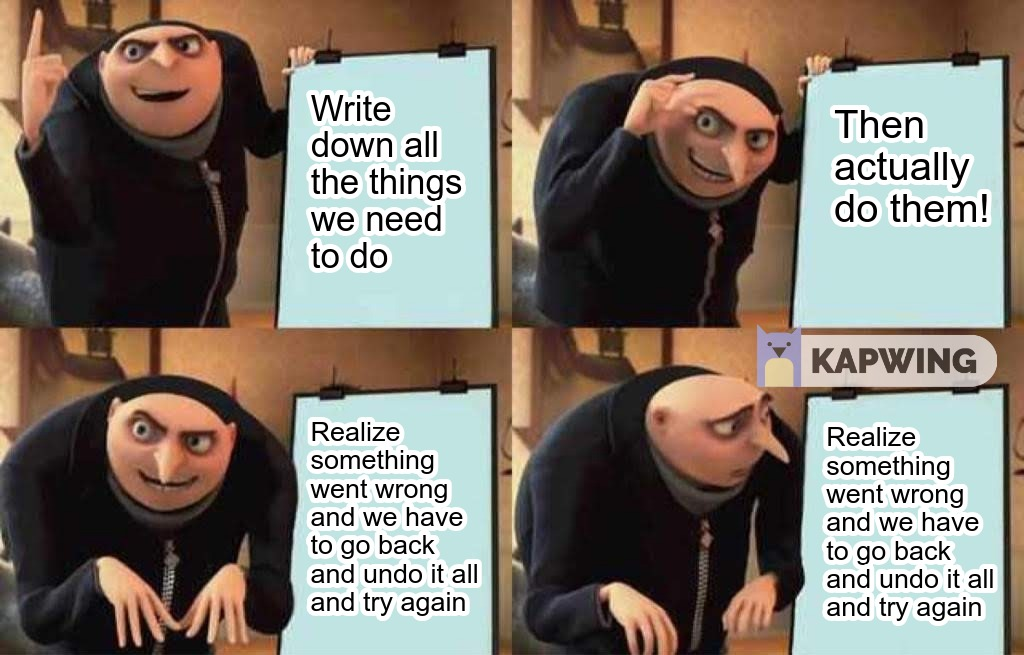
\includegraphics[width=0.9\textwidth]{images/gru-plan.jpg}
	\end{center}

\end{frame}



\begin{frame}
	\frametitle{Copy-Modify-Merge}

	In the case of version control, if there are merge conflicts then we are notified that the merge cannot take place until conflicts are resolved.

	But in file systems, the last write wins.

\end{frame}


\begin{frame}
	\frametitle{You have \textit{N} unread notifications...}

	I'm an inbox-zero kind of person so this picture hurts:

	\begin{center}
		
\includegraphics[width=\textwidth]{images/inbox-nonzero.jpg}
	\end{center}
	\hfill Image credit: Dhvanesh Adhiya

\end{frame}


\begin{frame}
	\frametitle{Notify Me}

	Another way that we can use the file system (in Linux only!) for synchronization or concurrency control is through the use of \texttt{inotify}.

	Using this API, you can register your program as being interested in the events.

	You say you want to watch a file or directory, and when an event occurs, then your program is informed

\end{frame}


\begin{frame}
	\frametitle{OVERWATCH!}

	The steps are:

	\begin{enumerate}
		\item Use an initialization function to create the management structure (and get a file descriptor back to refer to it).
		\item Then you tell the kernel what files you are interested in by adding them to the structure (you can also remove them).
		\item To collect an event, use \texttt{read} on the file descriptor. Each call returns one or more event structures.
		\item If you're done, close the file descriptor representing the management structure, which conveniently cleans everything up for you.
	\end{enumerate}

	The mechanism is not recursive.

\end{frame}

\begin{frame}[fragile]
	\frametitle{Notification API: Initialization}

	The API calls:
	\begin{lstlisting}[language=C]
int inotify_init( ); /* Returns file descriptor referring to the struct */
\end{lstlisting}

	Initialization doesn't require any arguments, so that's quite convenient.

\end{frame}

\begin{frame}[fragile]
	\frametitle{Notification API: Add}

	The API calls:
	\begin{lstlisting}[language=C]
int inotify_add_watch( int fd, const char* pathname, uint32_t mask );
\end{lstlisting}


	Adding an item to the watch takes as an argument the inotify structure to add it to, the name of the file to add, and a mask.

	You must have at least read permission on the file to be able to watch it.

	The mask is how we specify details about the events that we are interested in.

	We have to save the return value of the add function if we want to use the remove function.

\end{frame}

\begin{frame}[fragile]
	\frametitle{Notification API: Remove}

	The API calls:
	\begin{lstlisting}[language=C]
int inotify_rm_watch( int fd, uint32_t wd );
\end{lstlisting}

	Remove takes as an argument what was returned from add.

	When we're completely done, just call close on the file descriptor representing the inotify.

\end{frame}


\begin{frame}
	\frametitle{TV has so many channels...}

	There are about 23 different events that you can watch for using the bit mask.

	\begin{center}
		\begin{tabular}{l|l}
			\textbf{Bit Value}          & \textbf{Description}                             \\ \hline
			\texttt{IN\_ACCESS}         & File accessed (read/execute)                     \\
			\texttt{IN\_ATTRIB}         & Metadata changed, such as permissions            \\
			\texttt{IN\_CLOSE\_WRITE}   & File opened for writing was closed               \\
			\texttt{IN\_CLOSE\_NOWRITE} & File not opened for writing was closed           \\
			\texttt{IN\_CREATE}         & File or directory created in watched directory   \\
			\texttt{IN\_DELETE}         & File or directory deleted from watched directory \\
			\texttt{IN\_DELETE\_SELF}   & Watched file or directory deleted                \\
			\texttt{IN\_MODIFY}         & File modified (write, for example)               \\
			\texttt{IN\_OPEN}           & File opened                                      \\
			\texttt{IN\_ALL\_EVENTS}    & Watch for all of the above (and a few more)
		\end{tabular}
	\end{center}

\end{frame}


\begin{frame}[fragile]
	\frametitle{Well, Now What?}

	Imagine we have set up some files that we would like to watch.

	When ready for such an event, use \texttt{read} on the file descriptor for the inotify.

	If an event occurred, you get back a structure \texttt{inotify\_event}.

	\begin{lstlisting}[language=C]
struct inotify_event {
  int      wd;       /* Watch descriptor */
  uint32_t mask;     /* Mask describing event */
  uint32_t cookie;   /* Unique cookie associating related events (for rename(2))*/  
  uint32_t len;      /* Size of name field */
  char     name[];   /* Optional null-terminated name */
};
\end{lstlisting}

	Weird: the size of an inotify event is thus the structure size plus the length of the array, i.e.: \texttt{sizeof( struct inotify\_event) + len}.

\end{frame}


\begin{frame}
	\frametitle{Das ist Nicht Gut}

	Usually when we do a read we need to know how many bytes we'd like to read.

	If we're reading a struct, we know the size of the struct, but now it depends on the length of the data you get back.

	Your standard clairvoyance problem.

	One approach is to just make the buffer really big...

\end{frame}


\begin{frame}
	\frametitle{Consult an Expert?}

	\begin{center}
		
\includegraphics[width=0.5\textwidth]{images/clairvoyance.jpg}
	\end{center}

\end{frame}



\begin{frame}
	\frametitle{If you don't know, ask!}

	\texttt{ioctl} can tell you what you want to know!

	\texttt{ioctl( fd, FIONREAD, \&numbytes )} updates \texttt{numbytes} with the number of bytes currently available to read from the inotify instance.

	If multiple events occurred you can get multiple structures back (if your buffer is big enough).


\end{frame}

\begin{frame}[fragile]
	\frametitle{Example of using inotify}

	\begin{lstlisting}[language=C]
const char filename[] = "file.lock";

int main( int argc, char** argv ) {
  int lockFD;
  bool our_turn = false;
  
  while( !our_turn ) {
    lockFD = open( filename, O_CREAT | O_EXCL | O_TRUNC );
    if ( lockFD == -1 ) {
      printf( "The lock file exists and process %ld will wait its turn...\n",
       getpid() ); 
      int notifyFD = inotify_init( );
      uint32_t watched = inotify_add_watch( notifyFD, filename, IN_DELETE_SELF );
      
       /* Read the file descriptor for the notify -- we get blocked here
         until there's an event that we want */
      int buffer_size = sizeof( struct inotify_event ) + strlen( filename ) + 1;
      char* event_buffer = malloc( buffer_size );
      printf("Setup complete, waiting for event...\n");
      read( notifyFD, event_buffer, buffer_size );

\end{lstlisting}
\end{frame}


\begin{frame}[fragile]
	\frametitle{Example of using inotify}

	\begin{lstlisting}[language=C]     
      struct inotify_event* event = (struct inotify_event*) event_buffer;
      /* Here we can look and see what arrived and decide what to do.
         In this example, we're only watching one file and one type
         of event, so we don't need to make any decisions now */

      printf("Event occurred!\n");

      free( event_buffer );
      inotify_rm_watch( lockFD, watched );
      close( notifyFD );
    } else {
      char* pid = malloc( 32 );
      memset( pid, 0, 32 );
      int bytes_of_pid = sprintf( pid, "%ld", getpid() );

      write( lockFD, pid, bytes_of_pid ); 
      free ( pid );
      close( lockFD );
      our_turn = true; 
    }
  } 

  printf("Process %ld is in the area protected by file lock.\n", getpid());
  remove( filename );
  return 0;
}
\end{lstlisting}

\end{frame}

\begin{frame}
	\frametitle{Consistency Checking and Journalling}

	Unfortunately, an error, crash, or power failure or something similar may result in a loss of data or inconsistent data in the file system.

	The directory structures, pointers, inodes, et cetera are all data structures and if they become corrupted it may lead to serious problems.

	We may need to check for consistency:

	\begin{center}
		
\includegraphics[width=0.4\textwidth]{images/lab-testing.jpeg}
	\end{center}

\end{frame}

\begin{frame}
	\frametitle{Consistency Checking}

	We could check for inconsistent data periodically (e.g., on system boot up) and many operating systems do so.

	This is, of course, an operation that will consume a very large amount of time while the whole disk is scanned.

	UNIX: \texttt{fsck}. Windows: \texttt{chkdsk}/\texttt{scandisk}.

	These tools will look for inconsistent states (e.g., a file that claims to be 12 blocks but the linked list contains only 5) and will attempt to repair it.

	Its level of success depends on the nature of the problem and the implementation of the file system.

\end{frame}



\begin{frame}
	\frametitle{Preventing the Problem}

	Obviously we would like to prevent the problem, if we can.

	All modern OS file systems use transactions to ensure consistency.

	We'll talk about ZFS, APFS, and NTFS...

\end{frame}


\begin{frame}
	\frametitle{ZFS}

	ZFS uses the idea of transactions, making sure that the state is always consistent on disk.

	Much like the copy-modify-merge model, data is copied, then changed, then rewritten.

	Blocks are never overwritten with new data.

	Instead, a transaction writes all data and metadata to new blocks.

\end{frame}


\begin{frame}
	\frametitle{ZFS}

	Only when the transaction is complete, any references to the old blocks are replaced with the location of the new blocks.

	Then the old pointers and blocks can be cleaned up (reused or disposed of).

	Interesting weakness: what if the disk is totally full?!

\end{frame}

\begin{frame}
	\frametitle{APFS}

	Like some version control systems, APFS brings the ability to take snapshots of the file system.

	Freeze the state of the file system and from there any additional changes are ``diffs'' against that base state, meaning only new things take up space.

	This is potentially quite helpful for taking backups!


	... You do take backups, right?

\end{frame}


\begin{frame}
	\frametitle{Time Machine, Whyyyyy}

	The performance of your system can be degraded while traditional backups are being taken.

	Time-consuming: computing a diff between the last backup copy and the current.

	APFS approach is faster, but also a way to avoid corruption.

	You can replay changes as needed to get the file back to \textit{a} consistent.

\end{frame}


\begin{frame}
	\frametitle{More Copies, More Good?}

	The APFS does potentially harm the most common ``backup'' system of non-technical users: take a copy of the file and put it in a different folder.

	APFS will not actually duplicate the data on the same volume.

	It sounds like they're doing you a favour if you think of this as just reducing wasted space.

	But from the perspective of redundancy: if that part of the disk is damaged then all copies are lost.

\end{frame}

\begin{frame}
	\frametitle{Marketing-Speak, Engage}

	Somewhat like ZFS, the APFS approach to avoiding inconsistent data amidst a crash is something like copy-on-write.

	In typical Apple fashion they were pretty vague about what this means...

	The APFS lead developer Dominic Giampaolo just says it's a ``novel copy-on-write metadata scheme'' but also somehow not exactly the same as ZFS's single-atomic-update approach.

\end{frame}


\begin{frame}
	\frametitle{Example: NTFS (Windows File System)}

	NTFS uses several different storage levels:

	\begin{enumerate}
		\item \textbf{Sector}
		\item \textbf{Cluster}
		\item \textbf{Volume}
	\end{enumerate}


\end{frame}

\begin{frame}
	\frametitle{NTFS}

	The cluster is the fundamental unit of allocation of NTFS.

	This allows the file system to be independent of the size of physical sectors on the disk.

	A volume contains file system information, a collection of files, and free space.

	The logical volume may be some of a physical disk, all of one, or spread across multiple physical disks.

\end{frame}

\begin{frame}
	\frametitle{NTFS Volume Layout}

	\begin{center}
		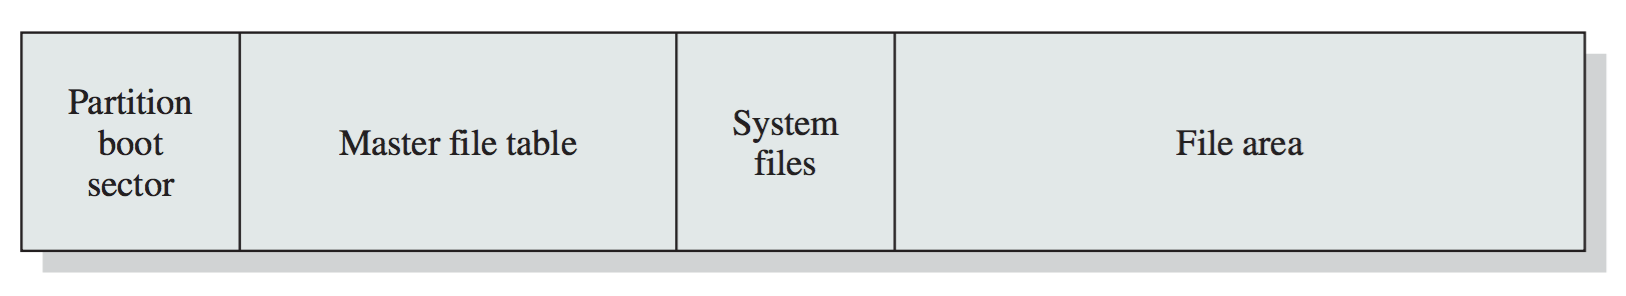
\includegraphics[width=0.9\textwidth]{images/ntfs-volume.png}
	\end{center}

\end{frame}

\begin{frame}
	\frametitle{NTFS System Files}

	The Master File Table (MFT) contains information about all the files and folders.

	A block is allocated to system files that contain important system information:

	\begin{enumerate}
		\item \textbf{MFT2}
		\item \textbf{Log File}
		\item \textbf{Cluster Bitmap}
		\item \textbf{Attribute Definition Table}
	\end{enumerate}
\end{frame}


\begin{frame}
	\frametitle{NTFS Journalling}

	NTFS uses journalling to ensure that the file system will be in a consistent state at all times, even after a crash or restart.

	There is a service responsible for maintaining a log file that will be used to recover in the event that things go wrong.

	Note that the goal of recovery is to make sure the system-maintained metadata is in a consistent state; user data can still get lost.

	This was a Microsoft design decision.

\end{frame}


\begin{frame}
	\frametitle{Sorry, You Lose}

	A particular write may not have taken place because of a crash, resulting in some data loss for you, the user.

	But at least the system will always remain in a consistent state.

	As a side benefit, we can sometimes re-order the writes to get better performance.


\end{frame}


\begin{frame}
	\frametitle{NTFS Journalling Implementation}

	The actual implementation of journalling:

	\begin{enumerate}
		\item Record the change(s) in the log file in the cache.
		\item Modify the volume in the cache.
		\item The cache manager flushes the log file to disk.
		\item Only after the log file is flushed to disk, the cache manager flushes the volume changes.
	\end{enumerate}

\end{frame}


\begin{frame}
	\frametitle{Just Deal with This}

	What's really interesting about this is that the changes are carried out in the background, that is to say, asynchronously.

	A program can say that it wants to write some data, and not have to wait for the data to be written before going on to the next thing.

	How interesting!

	Can we get that behaviour in our (regular) program? Yes we can...


\end{frame}





\end{document}
